\subsubsubsubsection{Scheduler}
\begin{figure}[h]
\centering
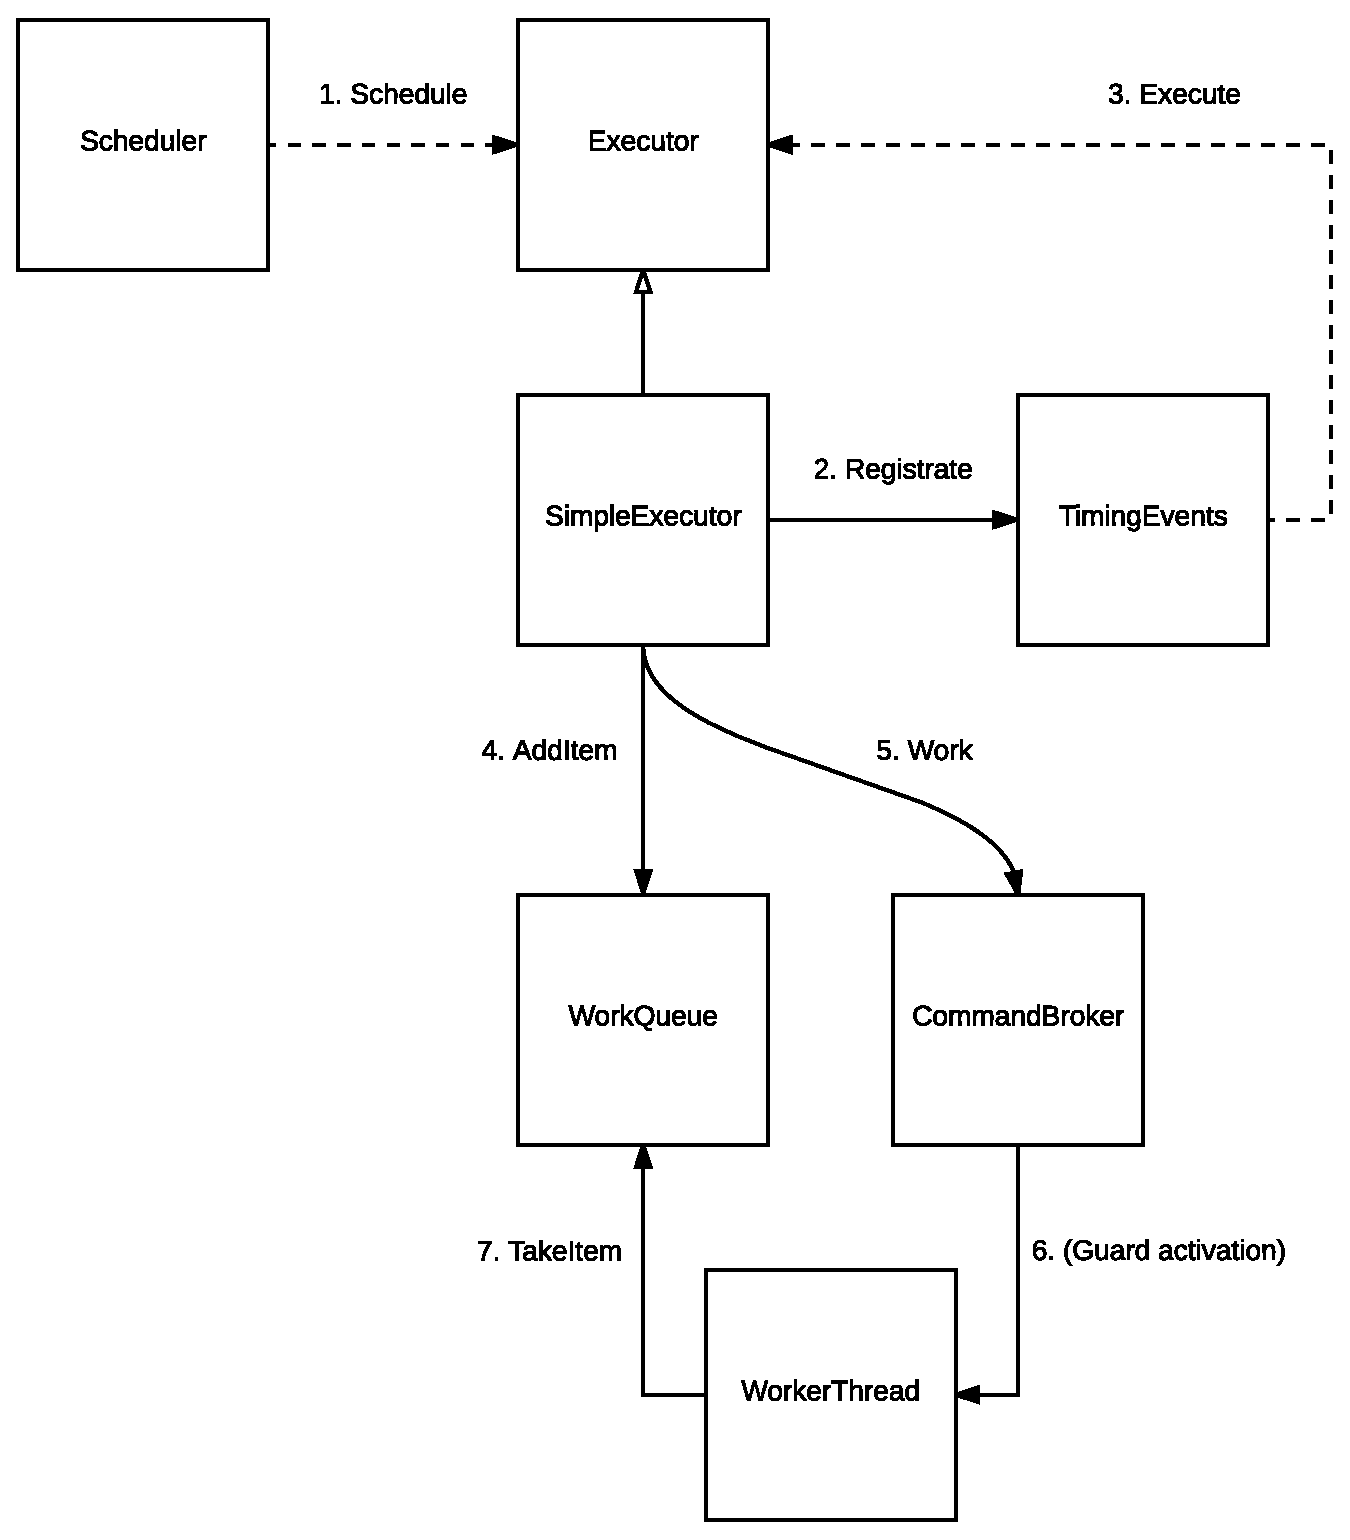
\includegraphics[scale=0.6,keepaspectratio]{images/solution/app/backend/scheduler.eps}
\caption{\pScheduling::Scheduler}
\label{fig:sd-app-scheduling-scheduler}
\end{figure}
\FloatBarrier
\begin{itemize}
  \item \textbf{\descr} \\
  An abstraction of a scheduler of travellers.
  Ensures the existence of at most one instance of a concrete ``Scheduler", 
  and provides a global point of access to it.
  Uses lazy initialization, hence no class instance is created 
  or stored until one is first requested.
  It is a singleton because only one traveller scheduler is needed.
  \item \textbf{\attrs}
  \begin{itemize}
    \item \texttt{\underline{instance : Scheduler = nil}} \\
    A static attribute that contains the unique instance 
    of a concrete \texttt{Scheduler}. It is initialized to nil.
    \item \texttt{agents: Collection<Agent>} \\
	A collection of travellers.
	\item \texttt{strategy: schedulingStrategy} \\
	A scheduling algorithm.
  \end{itemize}
  \item \textbf{\ops}
  \begin{itemize}
    \item[+] \texttt{\underline{getInstance() : Scheduler}} \\
    Static method lets clients access the unique instance 
    of \texttt{Scheduler}. At the first invocation, it is responsible 
    for creating the instance.
    \item[+] \texttt{setStrategy(strategy: schedulingStrategy)} \\
    Sets the scheduling algorithm.
    \item[+] \texttt{attach(agent: Agent)} \\
    Attaches an agent.
	\item[+] \texttt{detach(agent: Agent)} \\
	Detaches an agent.
	\item[+] \texttt{\textit{notify()}} \\
	An abstract method notifies of changes all the attached ``Agent'' objects.
  \end{itemize}
\end{itemize}
